%%%%%%%%%%%%%%%%%%%%%%%%%%%%%%%%%%%%%%%%%%%%%%%%%%%%%%%%%%%%%%%%%%% 
%                                                                 %
%                            CHAPTER                              %
%                                                                 %
%%%%%%%%%%%%%%%%%%%%%%%%%%%%%%%%%%%%%%%%%%%%%%%%%%%%%%%%%%%%%%%%%%% 

\chapter{Literature Review}
In this chapter, we will review the state of the art in the field of object counting. We will study the techniques commonly used for counting and go in more depth about the topic of few-shot object detection and why it should be applied to our problem. Finally, we will discuss the metrics used to evaluate the performance of the models.

\section{Crowd Counting}
Counting networks are an established concept in machine learning as numerous papers tackle the issue of counting humans, cars, animals or cells. What those have in common is that they only encompass a small set of possible categories to count and that, as they have a large real-life use, large annotated datasets exist like ShanghaiTech\cite{Shanghaitech} and COWC\cite{COWC}. The problem we are trying to solve is a bit different as we want to count a large set of objects and yet we don't have a large dataset to train on.

The methodology behind heuristic counting networks has three big streams\cite{s22145286}. The first applies a detection method to the image and then counts the number of detected objects. Many different detection methods can be used, from looking for characteristic features to matching the shape of the objects. The second takes a more global approach by first extracting features, textures, gradients and other information from the image as a whole and then using those to count the objects. The third method is not used on static images, but on video. It assumes that the objects are moving in clusters and uses that to predict the movement of the objects and improve detection.

Out of those three methods, the third one is not applicable to our problem as we are trying to detect unmoving objects in a still image.
Both the first and second methods are applicable to our problem, however, both have the problem of requiring a large dataset to train on. We will have to use a method that doesn't require a large dataset, which is where few-shot learning comes in. In the domain of few-shot learning the first method, object detection, is the most common. In the next section, we will go more in-depth about few-shot object detection.

%https://www.mdpi.com/1424-8220/22/14/5286

%https://openaccess.thecvf.com/content/CVPR2022W/L3D-IVU/papers/Ranjan_Vicinal_Counting_Networks_CVPRW_2022_paper.pdf

\section{Object detection basics}

\section{Few-shot object detection}
%https://arxiv.org/abs/2112.11699
%https://ieeexplore-ieee-org.kuleuven.e-bronnen.be/stamp/stamp.jsp?tp=&arnumber=1597116
%add a reference to the first paper that did it
Few-shot object detection is a technique that has been gaining popularity in the last few years, but interest in making a model to classify without a big annotated dataset appeared as early as 2008 with zero-shot learning in \citet{aaai08-132}. It allows us to train a model with few annotated images, which is useful in scenarios where it isn't possible to get a large annotated dataset. Few-shot attempts to mirror the way humans learn, during our life we come across many new objects and we are able to recognize them even though we only saw them a few times. We do this by drawing on our knowledge of other objects and using that to recognize the new object\cite{biederman1987recognition}. 

Different approaches to few-shot learning vary on a few characteristics
\begin{itemize}
	\item The type of architecture used
	\item The amount and type of data used
\end{itemize}

In this section, we will go over the different options for each of these characteristics.

\subsection{Method}

There are two different methodologies that can be applied to few-shot learning, transfer learning and meta-learning. Each of these has its own advantages and disadvantages. %add metric learning and data augmentation

\subsubsection*{Transfer learning}

Transfer learning is a technique that has been used for a long time in machine learning. It allows us to use a model that has been trained on a large dataset as a base and, with a few changes to mitigate the small size of the novel dataset in few-shot learning, finetune (the last layers) on a novel dataset. The advantages of this method are that it is relatively easy to implement and it is fast. One of the problems with this method is that, because of the small size of the novel dataset, the Region proposal network (RPN), which provides class-agnostic bounding boxes, can not be properly trained and can sometimes completely miss the novel object classes. Mitigations for this problem do, however, exist. \cite{DBLP:journals/corr/abs-2011-10142, VU2022104398, DBLP:journals/corr/abs-2105-09491, DBLP:journals/corr/abs-2103-05950,rs14143255}.

\subsubsection*{Meta-learning}

Meta-learning learns on a higher order of abstraction. Instead of learning how to detect objects it learns how to learn to detect objects. It does this with the help of a large dataset, by learning how to best extract and differentiate the features of its classes. Due to the dataset being large, this can then be applied to a novel dataset. It is best if the novel dataset is similar to the large dataset, as it will be able to generalize better. Practically meta-learning is most commonly done by introducing a support branch\cite{few-shot-comprehensive-survey}, displayed in figure \ref{fig:2_dualbranchmeta}. An advantage of this method is that it is better at the detection of alike novel classes due to the meta loss, a loss function on the support branch. %needs citation
The disadvantages are its complexity and that it is slower to train than transfer learning due to the aforementioned support branch. As the support branch is computed once after training, it is not significantly slower during inference.
%needs sauces

\begin{figure}[H]
	\centering
	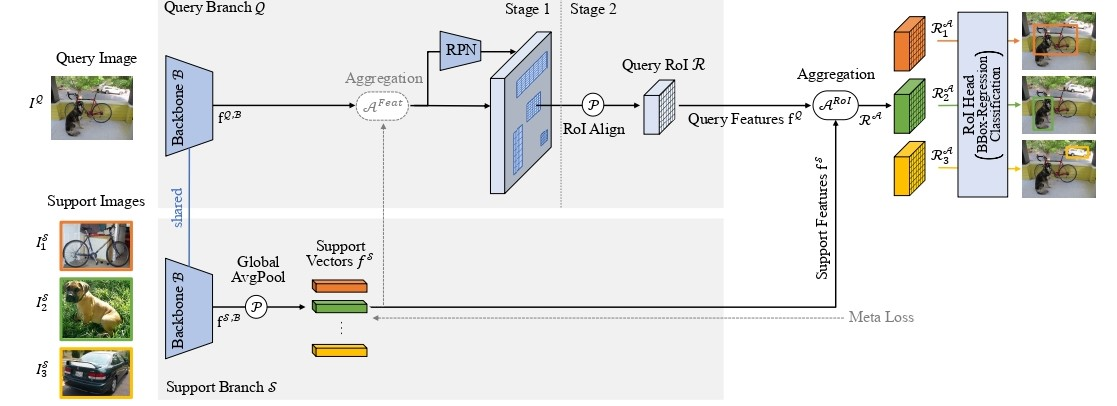
\includegraphics[width=1\textwidth]{2_dualbranchmeta}
	\caption{\label{fig:2_dualbranchmeta} Dual branch meta learning. Image from \citet{few-shot-comprehensive-survey}.}
\end{figure}

\subsection{Data}

The amount and type of data used in few-shot learning is also an important factor. A common way to describe a few shot task is "N-Way, K-Shot". Where N is the number of classes and K is the number of examples per class. The more examples we have per class, the easier it is to learn. The larger the number of classes the harder. Models are often benchmarked with increasing K to see how they perform with values of K often set at (2,) 5, 10 and 30. When the amount of images decreases even further we enter a whole new category of few-shot learning, one-shot learning and zero-shot learning. Finally, the requirements for the type of annotations on the data can vary depending on the training method used. Supervised requires a fully annotated dataset, semi-supervised a partially annotated dataset and unsupervised doesn't need labels at all.

\subsubsection*{One-shot learning}

While one-shot learning is not a new concept, applying it to object detection is hard. Early applications used a siamese backbone, as is often seen in other one-shot applications, but this was not very successful \citep{One-shot-siamese}. However, recently OWL-ViT \citep{owlvit} improved one-shot object detection by a large margin, reaching 41.8 mAP for one-shot object detection on the COCO dataset.


\section{Metrics}
In machine learning, it is important to test the model after training, to evaluate its performance. To test the model's accuracy a part of the initial dataset is split off into a test set and never used when training. As we have the ground truth for the test set we can compare it with the network output to find if the detections are correct. 

To find if the model output matches the expected output we use the Intersection over Union (IoU) metric. This compares the area of the input and output bounding boxes for each detection by dividing the area of intersection by the area of union. If the IoU, calculated as shown in \ref{eq:IoU}, is above a threshold (th) it is considered a detection.

\begin{figure}[h]
	\centering
	\documentclass{standalone}

\usepackage{tikz,pgf}

\begin{document}


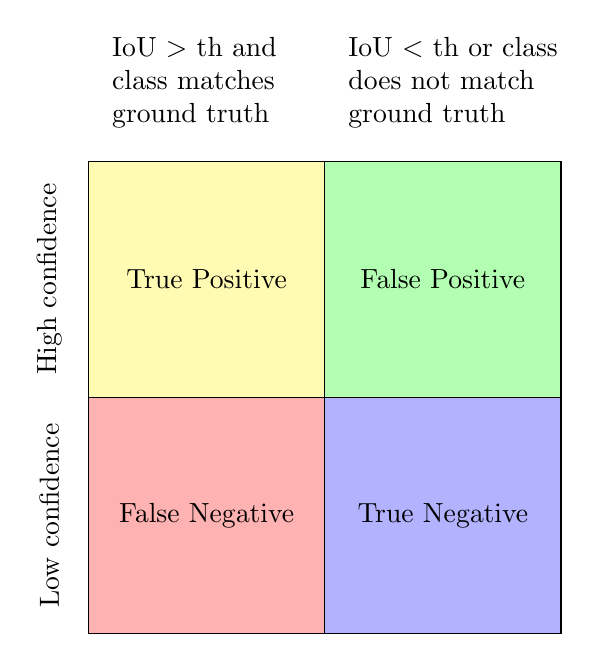
\begin{tikzpicture}
    \draw[draw=black,fill=yellow!30] (0,0) rectangle (3,3);
    \draw[draw=black,fill=green!30] (3,0) rectangle (6,3);
    \draw[draw=black,fill=red!30] (0,-3) rectangle (3,0);
    \draw[draw=black,fill=blue!30] (3,-3) rectangle (6,0);
    
    \node at (1.5,1.5) {True Positive};
    \node at (4.5,1.5) {False Positive};
    \node at (1.5,-1.5) {False Negative};
    \node at (4.5,-1.5) {True Negative};

    \node[text width=2.8cm] at (1.7,4) {IoU \begin{math}>\end{math} th and class matches ground truth};
    \node[text width=2.8cm] at (4.7,4) {IoU \begin{math}<\end{math} th or class does not match ground truth};
    \node[rotate=90] at (-0.5,1.5) {High confidence};
    \node[rotate=90] at (-0.5,-1.5) {Low confidence};
\end{tikzpicture}


\end{document}
	\caption{\label{fig:2_IoU_det} IoU and class match to find the type of detection.}
\end{figure}

\begin{equation}
	\text{IoU} = \frac{\text{area of intersection}}{\text{area of union}}
	\label{eq:IoU}
\end{equation}

Each detection can be put into one of four categories, based on if and how well it matches the ground truth, listed below.

\begin{itemize}
	\item True positive: The model correctly detects an object and the IoU is above the threshold.
	\item False positive: The model detects an object but the IoU is below the threshold or the model mislabels the object.
	\item False negative: The model does not detect an object but it should have.
	\item True negative: The model does not detect an object and it should not have, this is not used in the metrics as it is not very useful.
\end{itemize}

Using this a few key metrics can be calculated. The main metrics we will use are precision, recall and their derivatives. Precision (\ref{eq:precision}) is the ratio of true positives to the total number of positives. Recall (\ref{eq:recall}) is the ratio of true positives to the total number of detectable positives.



\begin{equation}
	Precision = \frac{TruePositives}{True Positives + False Positives}
	\label{eq:precision}
\end{equation}

\begin{equation}
	Recall = \frac{True Positives}{True Positives + False Negatives}
	\label{eq:recall}
\end{equation}

The threshold between high and low confidence can be chosen, a high threshold will result in a low recall but high precision. A low threshold will result in a high recall but low precision. Plotting the precision and recall against the threshold results in a precision-recall curve.

Averaging the precision across all recall levels results in the average precision (AP) metric. Averaging the AP over all classes results in the mean average precision (mAP) metric. The mAP is the most common metric used to evaluate object detection models.

\section{State of the art}
In this section, we will go over the state of the art in few-shot object detection with a focus on the previously discussed methods and types of data.

%Oneshot learning: https://arxiv.org/pdf/2205.06230v2.pdf
\subsection*{Simple Open-Vocabulary Object Detection
with Vision Transformers. (\citet{owlvit})}

\citet{owlvit} introduce a new method, Vision Transformer for Open-World Localization, or OWL-ViT. It uses recent developments in language encoders and contrastive image-text training, using both positive and negative examples of image-text pairs to divide the feature space. These models are trained on loosely matched image-text pairs, which can be abundantly found on the internet. They start from the Vision Transformer (ViT) architecture and pre-train it on a large dataset of these image-text pairs. The token pooling layer downsamples the output embeddings to optimize computation, for open-vocabulary detection this does not work, however. The token pooling layer is thus replaced with a set of lightweight classification and box heads at each output token. The classification head does a linear projection, while the box head is a simple MLP with one hidden layer with a gelu activation function. The whole model (both text and image encoders) is then finetuned on standard object detection datasets. It is then ready to be used for one-shot object detection as it can take text, but also image-derived embeddings to find matching objects in the query image.

Special characteristic: 1-Shot-N-Way without retraining.

Results: 41.8 AP50 on COCO one-shot object detection.

Notes: The performance of OWL-ViT has to be tested to see how well it performs on our shell dataset as the pretraining likely doesn't cover this area well. If it works well on a one-shot test, we could finetune it further on our dataset.

\begin{figure}[h]
	\centering
	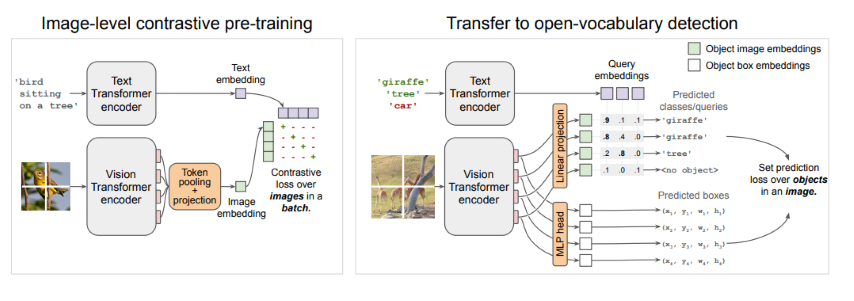
\includegraphics[width=1\textwidth]{2_owlvit.png}
	\caption{\label{fig:2_owl-vitr} Original ViT to OWL-ViT. Image from \citet{owlvit}.}
\end{figure}

%K-shot(10), DETR, transfer learning, unsupervised: https://arxiv.org/pdf/2106.04550v4.pdf



%K-shot(30), ViT, transfer learning from self-supervised, fully-supervised: https://arxiv.org/pdf/2205.09613v2.pdf
\subsection*{Integrally Migrating Pre-trained Transformer Encoder-decoders
for Visual Object Detection. (\citet{imTED})}

\citet{imTED} extend the ViT architecture by making full use of the transformer encoder-decoder instead of merely using the encoder as its backbone, as many other methods do. Whereas other methods use the encoder as their backbone and initialize the FPN, RPN and detector head from scratch, imTED instead uses the decoder as its detector head. As such the only parts that need to be trained are the FPN, RPN and output layers of the FPN and decoder. This reduces the number of parameters that are randomly initialized by 81.3\%.

Results: SOTA on COCO 30-shot object detection with 30.2 AP.

\begin{figure}[h]
	\centering
	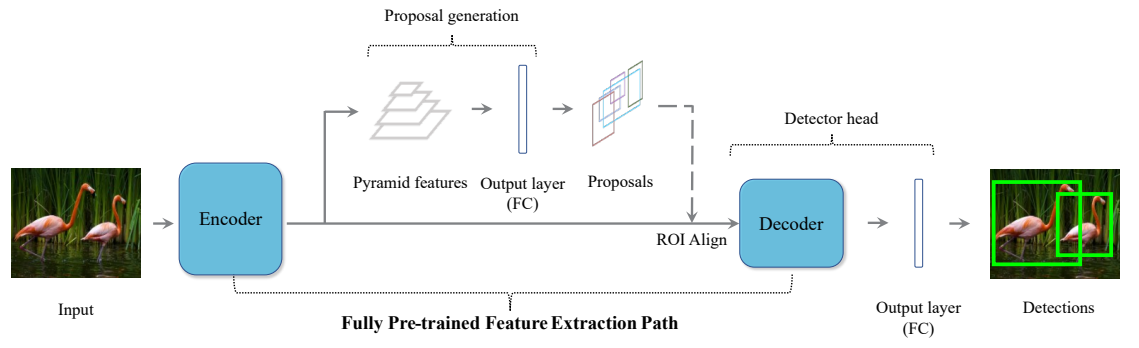
\includegraphics[width=1\textwidth]{2_imTED_full}
	\caption{\label{fig:2_imTED_full} imTED architecture. Image from \citet{imTED}.}
\end{figure}

%K-shot, Faster R-CNN, meta-learning: https://arxiv.org/pdf/2208.07039v3.pdf
\subsection*{Hierarchical Attention Network for Few-Shot
Object Detection via Meta-Contrastive Learning. (\citet{hANMCL})}

\citet{hANMCL} expand upon Faster R-CNN \citep{fasterrcnn} by introducing a  hierarchical attention module (HAM) and a meta-contrastive learning module (Meta-CLM). The HAM combines the robustness of global attention with the local context information of a convolutional network by first applying local attention and then applying global attention. The stages can be found in fig \ref{fig:2_hANMCL_HAM}. The Meta-CLM combines contrastive learning with meta-learning. It works on the same principles as contrastive learning, only instead of positive and negative images it uses positive and negative image pairs. Due to being metric-based, it can be used without any finetuning on novel classes.

Special characteristic: As opposed to many other SOTA methods, this method does not use vision transformers.

Results: 22.4 AP on COCO 10-shot object detection, 25 AP on COCO 30-shot object detection.

Notes: This model can be used without finetuning for novel classes, much like OWL-ViT. Due to its small size, it can be trained on less powerful hardware. As it uses metric-based meta-learning, it shows potential for our problem of alike shells.

\begin{figure}[H]
	\centering
	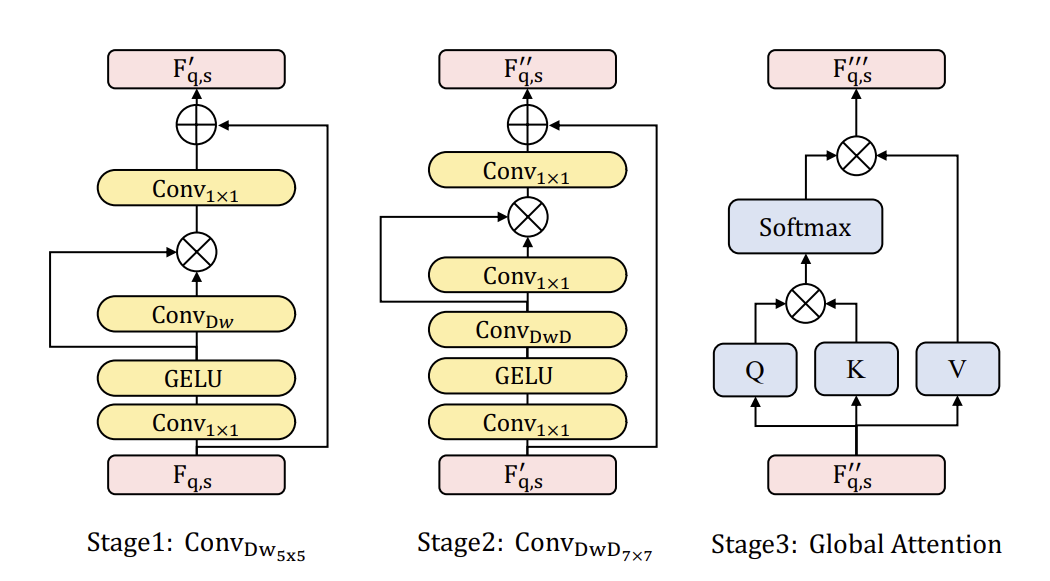
\includegraphics[width=0.8\textwidth]{2_hANMCL_HAM.png}
	\caption{\label{fig:2_hANMCL_HAM} Detailed view of the HAM. Image from \citet{hANMCL}.}
\end{figure}

\begin{figure}[H]
	\centering
	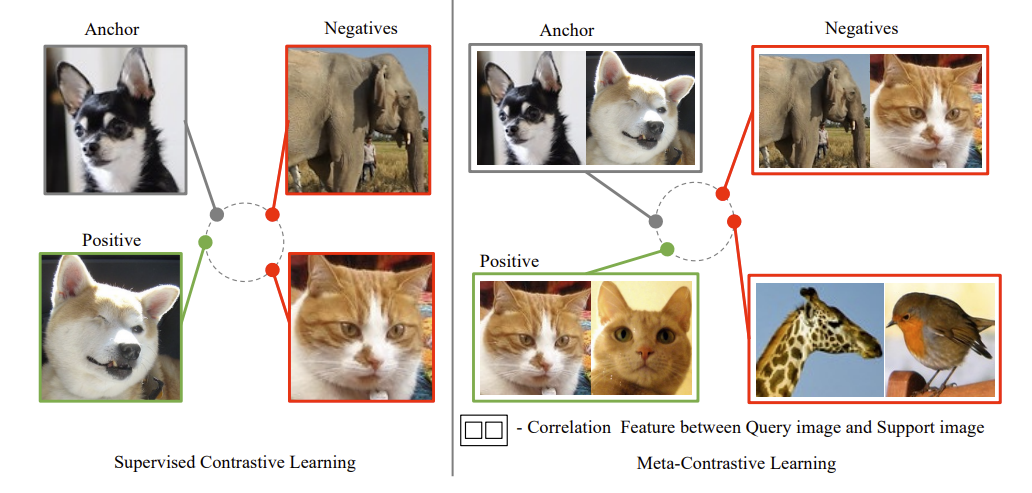
\includegraphics[width=0.8\textwidth]{2_hANMCL.png}
	\caption{\label{fig:2_hANMCL} Meta-contrastive learning. Image from \citet{hANMCL}.}
\end{figure}

\section{Conclusion}
In this chapter we have studied object counting, narrowing it down to few-shot object detection to then count the detections. We went into more detail regarding the different ways to implement few-shot learning to detect objects. The sub-field of meta-learning shows the most promise for our problem as it is better at learning the difference between two alike novel classes compared to transfer learning.